\begin{figure*}
	\tikzset{
		%Define standard arrow tip
		>=stealth',
		%Define style for boxes
		punkt/.style={
				rectangle,
				rounded corners,
				draw=black, very thick,
				text width=6.5em,
				minimum height=2em,
				text centered
			},
	}
	\begin{adjustbox}{width=\textwidth}
		\begin{tikzpicture}

			\node[] (z) {$z \sim \operatorname{N}(0,1)$};
			\node[circle, draw, thick, right=5em of z] (x) {$\vec{x}_{fake}$};
			\draw[-stealth, thick] (z) -- node[above] {$G(\vec{z})$} node[below] {generator} (x);
			\node[left=of z] (i) {};
			% \draw[-stealth, thick] (i) -- node[above] {$p_\theta(\vec{z})$} (z);
			\node[above=of x, circle, draw, thick] (xt) {$\vec{x}_{real}$};
			\node[left=5em of xt] (it) {};
			\draw[-stealth, thick] (it) -- node[above] {$p_{data}(\vec{x})$} (xt);
			\node[circle, draw, thick, right=5em of x, yshift=2.5em] (D) {$\vec{x}$};
			\node[right=7em of D] (out) {real?};
			\draw[-stealth, thick] (D) -- node[above] {$D(\vec{x})$} node[below] {discriminator} (out);

			\node[right=2.5em of x, circle, fill, inner sep=0.15em] (pt1) {};
			\node[right=2.5em of xt, circle, fill, inner sep=0.15em] (pt2) {};

			\draw[dashed, thick] (pt1) edge[bend left] (pt2);

			\node[circle, draw, thick, fill=white, inner sep=0.15em] at ([xshift=-0.9em, yshift=4em]pt1.north) (pt3) {};

			\draw[-stealth, thick] (x) -- (pt1);
			\draw[-stealth, thick] (xt) -- (pt2);
			\draw[-stealth, thick] (pt3) -- (D);

		\end{tikzpicture}
		% Define block styles
		% \tikzstyle{decision} = [diamond, draw, fill=blue!20, 
		% text width=4.5em, text badly centered, node distance=3cm, inner sep=0pt]
		% \tikzstyle{block} = [rectangle, draw, fill=blue!20, 
		% text width=5em, text centered, rounded corners, minimum height=4em]
		% \tikzstyle{line} = [draw, -latex']
		% \tikzstyle{cloud} = [draw, ellipse,fill=red!20, node distance=3cm,
		% minimum height=2em]

		% \begin{tikzpicture}[node distance = 2cm, auto]
		% % Place nodes
		% \node [block] (init) {initialize model};
		% \node [cloud, left of=init] (expert) {expert};
		% \node [cloud, right of=init] (system) {system};
		% \node [block, below of=init] (identify) {identify candidate models};
		% \node [block, below of=identify] (evaluate) {evaluate candidate models};
		% \node [block, left of=evaluate, node distance=3cm] (update) {update model};
		% \node [decision, below of=evaluate] (decide) {is best candidate better?};
		% \node [block, below of=decide, node distance=3cm] (stop) {stop};
		% % Draw edges
		% \path [line] (init) -- (identify);
		% \path [line] (identify) -- (evaluate);
		% \path [line] (evaluate) -- (decide);
		% \path [line] (decide) -| node [near start] {yes} (update);
		% \path [line] (update) |- (identify);
		% \path [line] (decide) -- node {no}(stop);
		% \path [line,dashed] (expert) -- (init);
		% \path [line,dashed] (system) -- (init);
		% \path [line,dashed] (system) |- (evaluate);
		% \end{tikzpicture}


		% 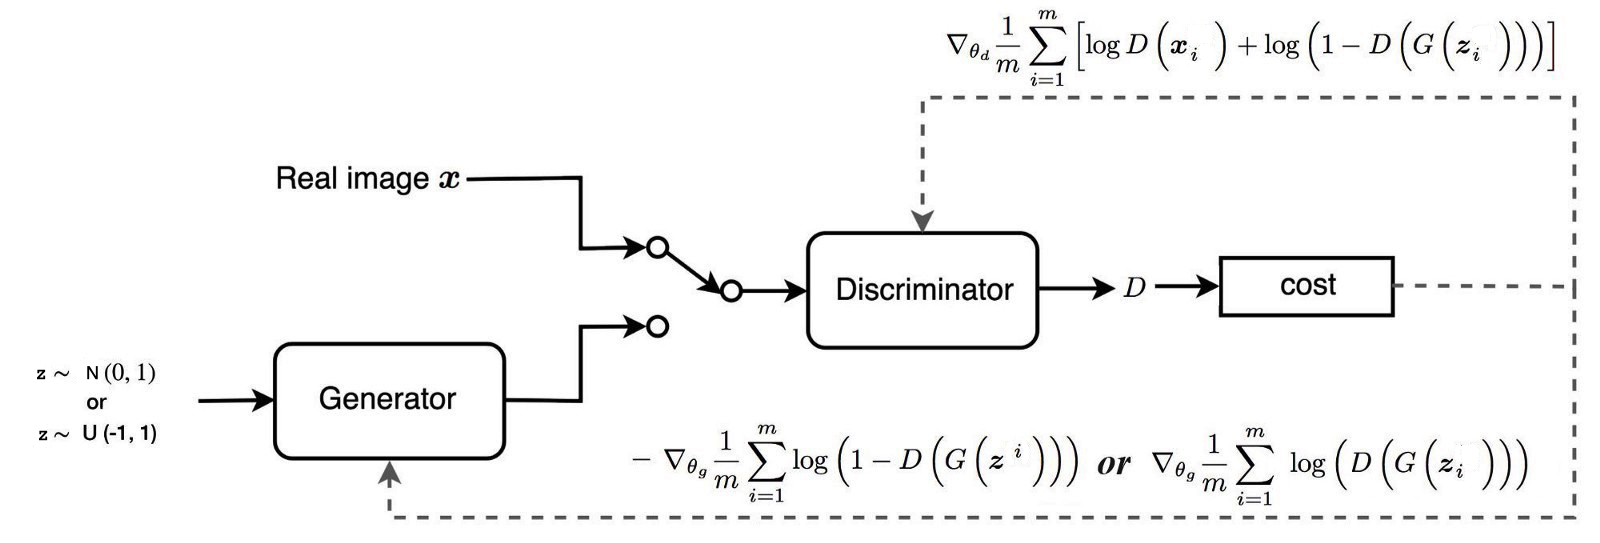
\includegraphics[]{figures/neural_networks/gan.jpeg}
	\end{adjustbox}
	\caption{Schematic diagram for Generative Adversarial Network\cite{ponti2017}.}\label{fig:gan}

\end{figure*}
\begin{figure*}
	\begin{adjustbox}{width=\textwidth}
		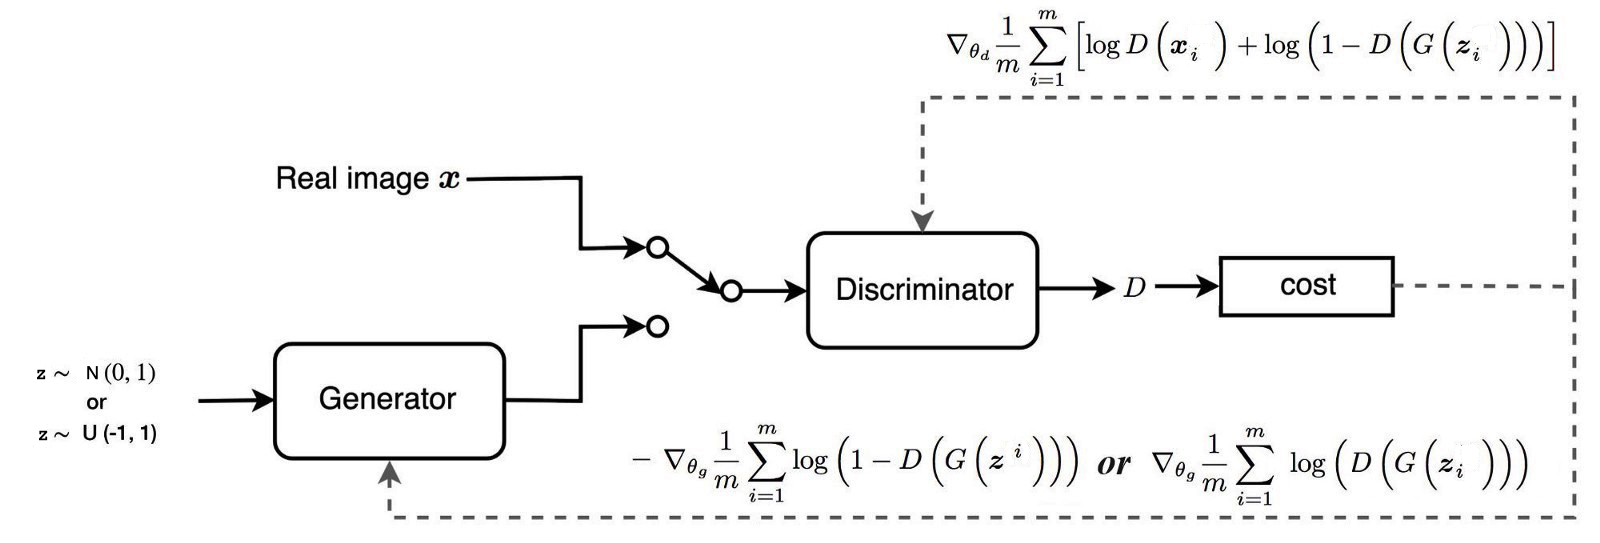
\includegraphics[]{figures/neural_networks/gan.jpeg}
	\end{adjustbox}
	\caption{Schematic diagram for Generative Adversarial Network\cite{ponti2017}.}\label{fig:gan}

\end{figure*}

